%%This section presents any experiments or analyses that are needed
%%to support the technical quality of the dataset. This section may
%%be supported by up figures and tables, as needed. This is a required
%%section; authors must present information justifying the reliability
%%of their data.

\section{Technical validation}

\subsection{Comparison to other data bases}

We sampled an entry for each of the 50 most occurring concentration units and compared the Standartox conversions to manually calculated conversions for these, to guarantee the correctness of unit conversions. The same was done for six samples of duration units (See \ref{tab:chck-unit}

To guarantee correctness of unit conversions we sampled an entry for each of the 50 most frequent concentration units. and the six most frequent duration units, respectively.

Out of the 1229 concentration units in the EPA ECOTOX data base, Standartox retains only those (n = X) whih are convertible to one of the following units: ug/l, ul/l, ppb, g/m2, mg/kg, \%, resulting in 873473 out of 952625 test results. Likewise, out of the 125 test duration units in the EPA ECOTOX, Standartox retains only those (n = X) which are accurately convertible to hours, leading to 905110 out of 952625 test results (see table \ref{tab:units-duration}). % TODO 

The here described Standartox version uses the EPA ECOTOX data base released on the 12.09.2019.


In order to asses the validity of the Standartox approach to aggregate test results we compared Standartox values with effect values for the same chemicals and the same test duration from the PPDB (n=3601) \ref{fig:standartox_ppdb_diff}. This showed that 91.3\% of the Standartox values diverge by less than a factor of 10 from the PPDB values. Considering only Standartox values for which at least five of ten tests were aggregated the value increases to 91.7\% and 93.4\% respectively. Admittedly a few Standartox values diverge by a large margin.

\begin{figure}
    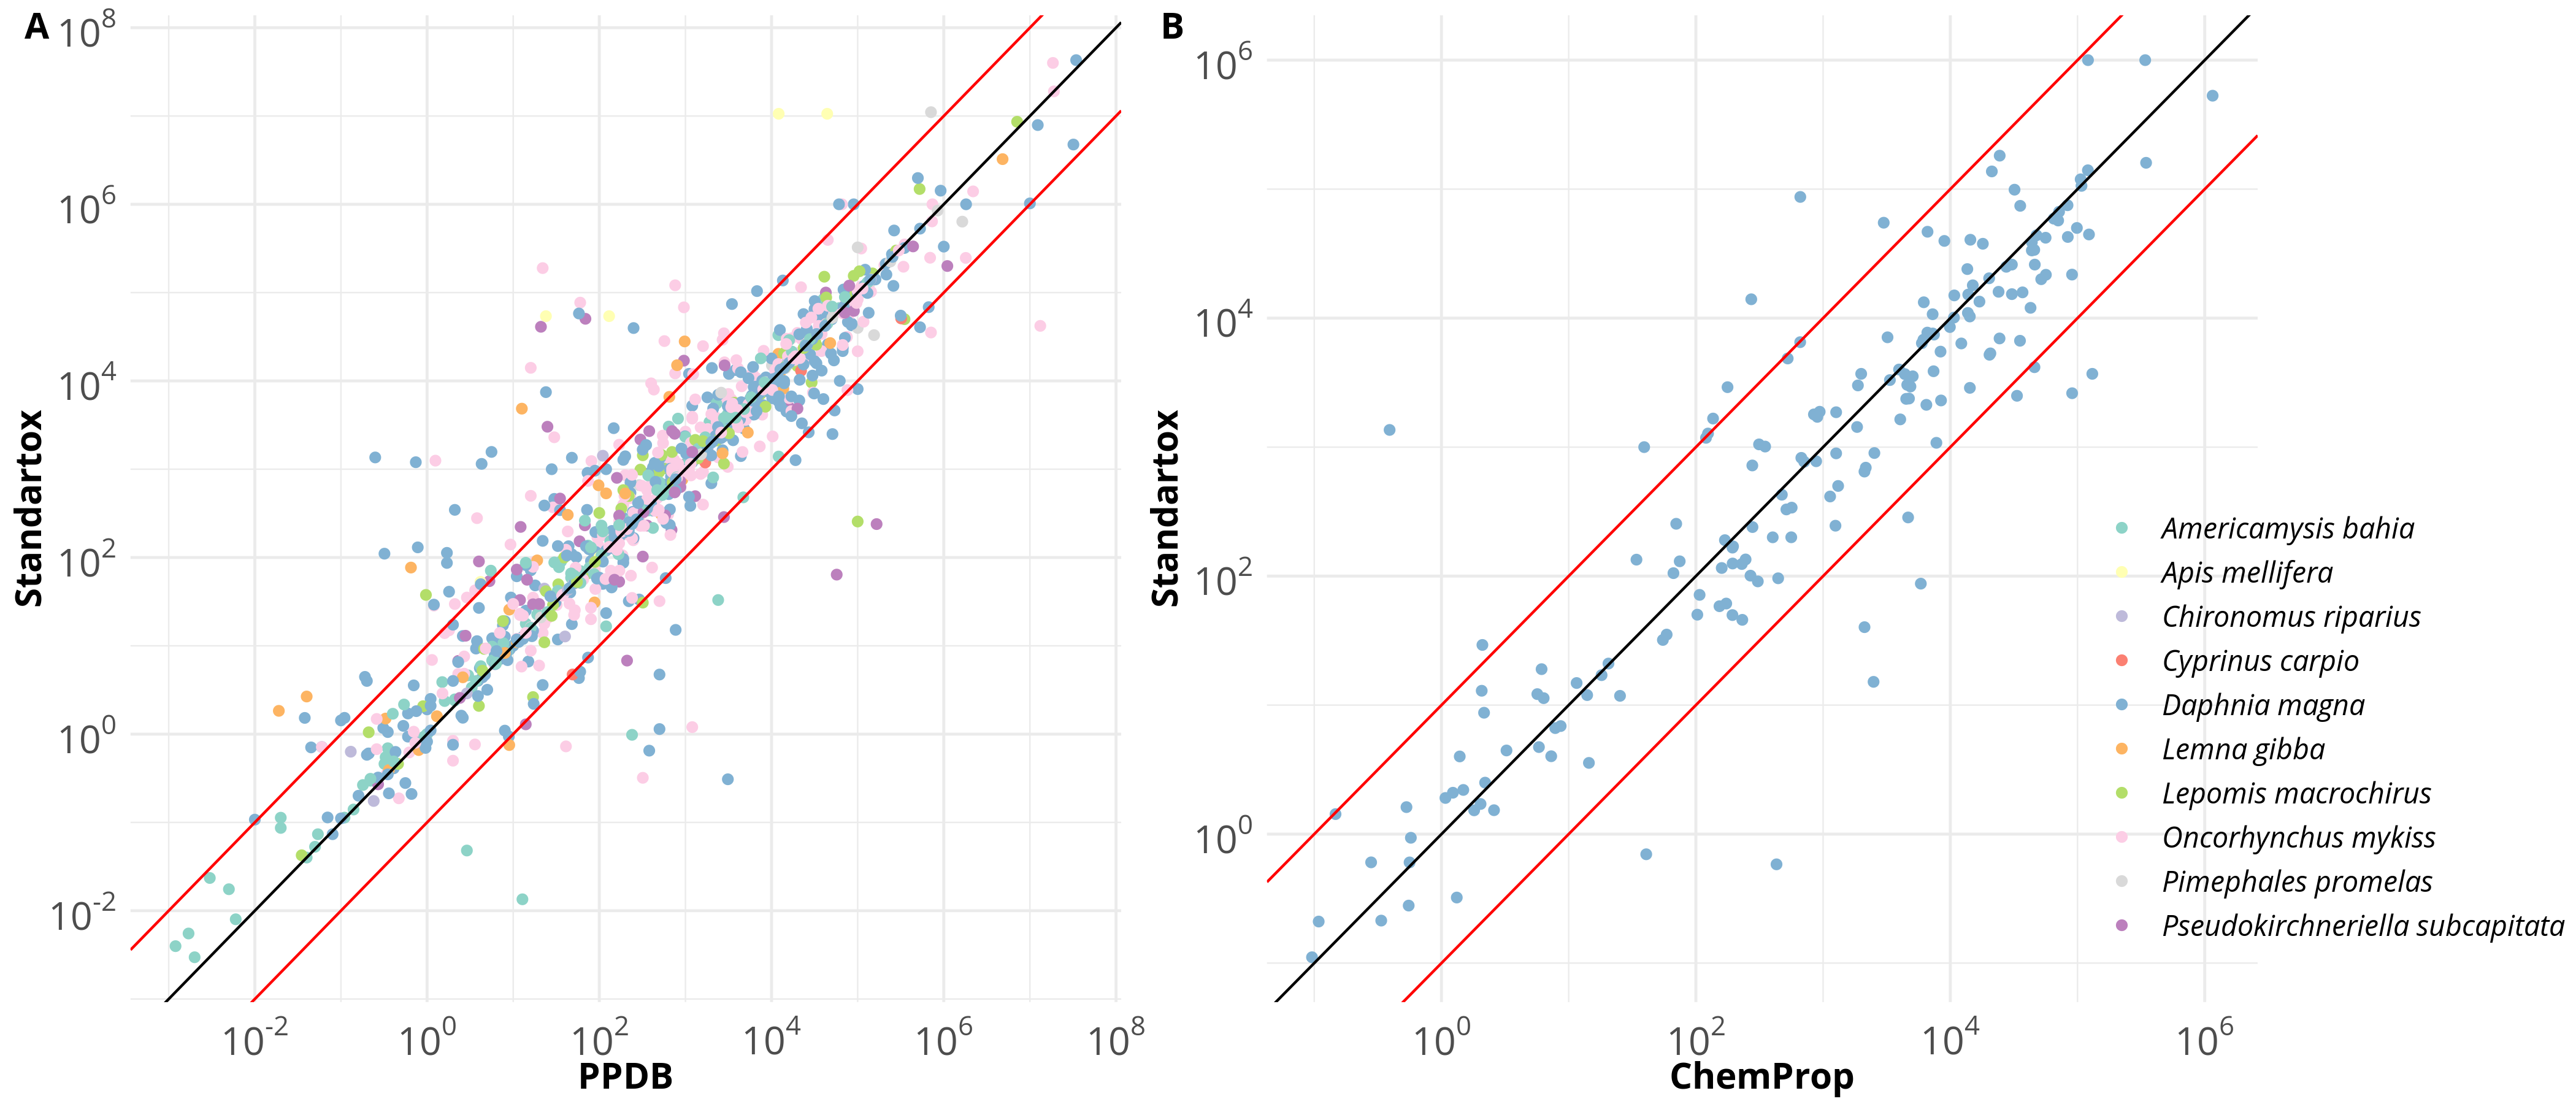
\includegraphics[width=1\linewidth]{article/figures/gg_ppdb_stan_compare_continous.png}
    \caption{Comparison between Standartox and PPDB values}
    \label{fig:standartox_ppdb_diff}
\end{figure}

\subsection{Unit Harmonisation}

In order to assure appropriate conversion and harmonisation of units we took a random sample of the 50 most occurring units and converted them manually and subsequently compared them to the conversions done by Standartox.

We did this for concentration units and duration units

in R/chck\_unit\_conversion.R


\subsection{Overall distribution of tests}
Heatmap: don't Include for now. Too large.
Put maybe a plotly on wep app
Mybe search for the 50 most sold chemicals and asses the number of tests


In order to validate Standartox we compared resulting values with values from other data bases, such as the PPDB. Of 542 chemicals, only 16\% diverged from the PPDB values by a factor greater than 10, supporting plausibility of the \standartox results \ref{fig:standartox_ppdb_diff}.


